% !TEX = root../thesis.tex

\chapter{Experimental Apparatus}
\label{chap:exp}

\section{The Large Hadron Collider} \label{sec:LHC}
% Overview
The Large Hadron Collider (LHC) is a circular collider spanning the border between France and Switzerland, based at the European Organization for Nuclear Research (CERN). The central features of the LHC are the superconducting rings, located about 100 m underground with a circumference of 27 km, designed to collide counter-rotating beams of protons or heavy ions at highly relativistic energies. Along the rings lie four major experiments: ATLAS, CMS, ALICE, and LHCb. Both ALTAS and CMS are general purpose detectors, designed to probe a wide range of physics including the Higgs boson, precision measurements of fundamental constants, and physics beyond the standard model (BSM). The remaining two experiments are more specialized; ALICE measures quark gluon plasma produced in heavy ion collisions and LHCb focuses on $b$-quark physics and CP violation.

% Lumi and CoM energy
Two prominent aspects of the LHC are the high center of mass energy, referred to using the Mandelstam variable $\sqrt{s}$, and high instantaneous luminosity $\lumi$, often referred to as just luminosity. High $\sqrt{s}$ allows for the production of more massive particles, giving more access to possible BSM physics, while high luminosity is essential for measuring rare processes and precision measurements. A process with cross section $\sigma$ will have a rate $R$ given by
\begin{equation}
	R=\lumi\sigma
\end{equation}

The cross section $\sigma$ is a measure of how probably a process is to occur, and is in units of area. They are frequently measured in $\unit{barns}$, where $1\unit{b} = 100\unit{fm^2}$. Conversely, luminosity uses units of $\unit{Hz/b}$. In cases where the relevant quantity is the total number of events, the integrated luminosity can be defined as $\intlumi=\int{\lumi\dd{t}}$ to give
\begin{equation}
	N_\mathrm{events} = \intlumi\sigma
\end{equation}

The luminosity depends on the characteristics of the proton beam and can be written in terms of the operational parameters of the detector given by
\begin{equation}
	\lumi=\frac{N_b^2n_bf_\mathrm{rev}\gamma_r}{4\pi\epsilon_n\beta^*}F
\end{equation}
where $N_b$ is the number of particles per bunch, $n_b$ is the number of bunches per ring, $f_\mathrm{rev}$ is the LHC revolution frequency, $\gamma_r$ is the Lorentz factor for the proton, $\epsilon_n$ is the transverse normalized beam emittance, $\beta^*$ is the amplitude function at the collision point, and $F$ is a geometric reduction factor based on the crossing angle of the two beams. The nominal design parameters of the LHC were intended to support a peak luminosity of $12\unit{Hz/nb}$~\cite{Bruning:782076}, but were exceeded by nearly twice that value of $20.7\unit{Hz/nb}$ during 2017 data taking and again by $21.4\unit{Hz/nb}$ in 2018. The LHC produced $41.6\unit{fb^{-1}}$ in 2016, $49.8\unit{fb^{-1}}$ in 2017, and $67.9\unit{fb^{-1}}$ in 2018 for a total of $159.3\unit{fb^{-1}}$ during run 2 data taking. A more detailed breakdown of the LHC luminosity records can be seen in Fig.~\ref{fig:LHC_lumi}.

\begin{figure}[!htbp]
	\centering
	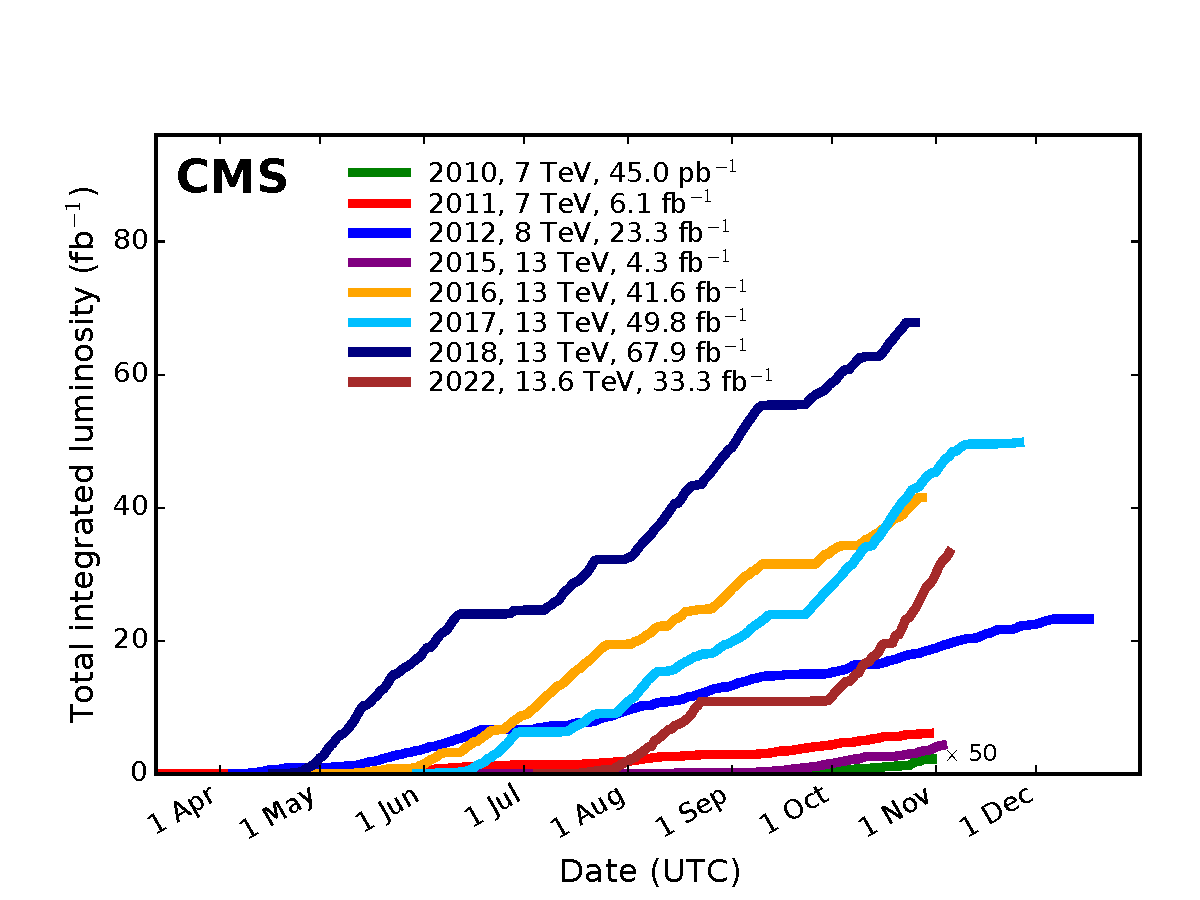
\includegraphics[width=0.34\textwidth]{figs/03_experiment/int_lumi_cumulative_pp_2.pdf}
	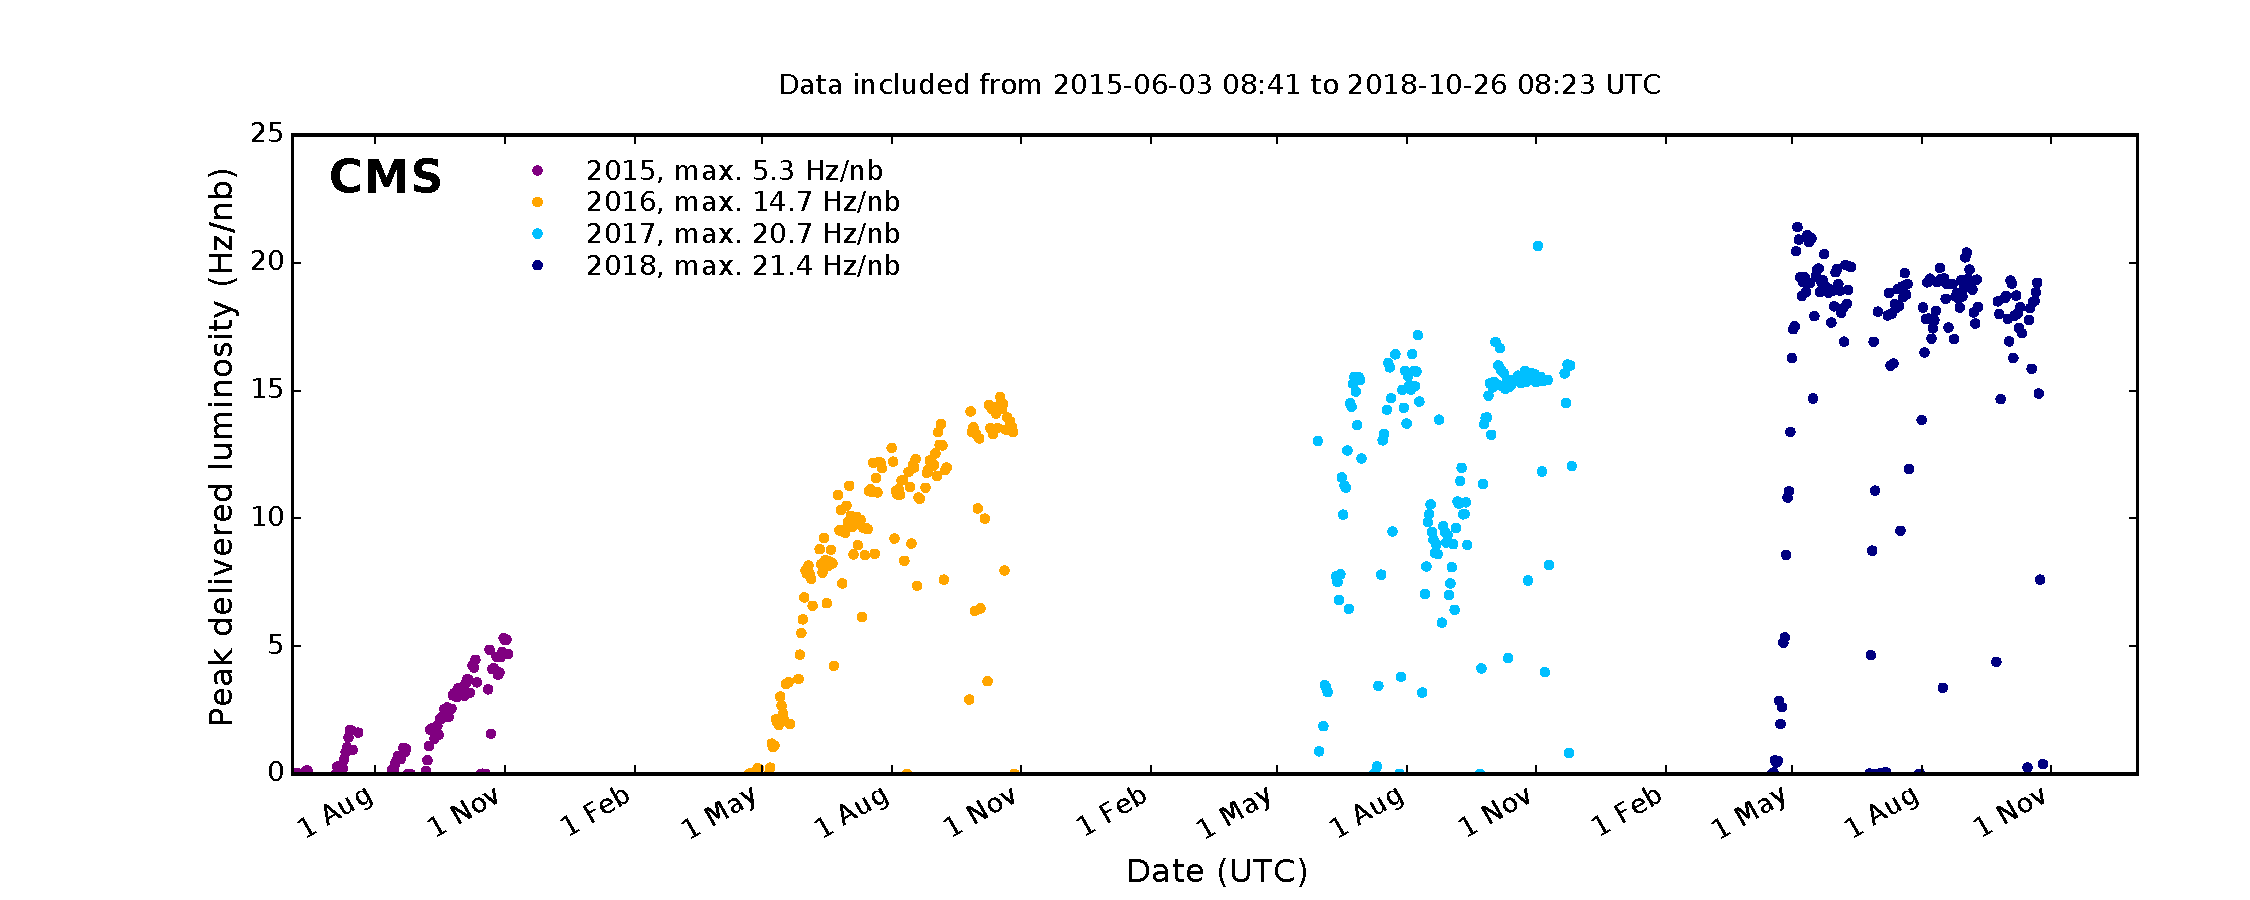
\includegraphics[width=0.65\textwidth]{figs/03_experiment/peak_lumi_pp_run2.pdf}
	\caption[LHC luminosity report. Left: breakdown of the CMS integrated luminosity by year from 2010-2022. Right:  peak luminosity from 2016-2018 data taking~\cite{CMSlumi}.]
	{LHC luminosity report. Left: breakdown of the CMS integrated luminosity by year from 2010-2022. Right: peak instantaneous luminosity from 2016-2018 data taking~\cite{CMSlumi}}
	\label{fig:LHC_lumi}
\end{figure}

\begin{comment} % Check these numbers? pdg values do not give the correct lumi
\begin{table}[htb!]
	\caption{Description of beam parameters used to calculate the LHC luminosity, obtained from~\cite{Workman:2022ynf} and~\cite{Herr:941318}}
	\begin{center}
		\begin{tabular}{l l l}
			\hline
			Parameter & Description & Value \\
			\hline
			$N_b$ & Number of particles per bunch & $1.1\times10^{11}$\\
			$n_b$ & Number of bunches per event & $2556$\\
			$f_\mathrm{rev}$ & Revolution frequency & $11.245\unit{kHz}$\\
			$\gamma_r$ & Lorentz factor & $6929.6$\\
			$\epsilon_n$ & Transverse normalized beam emittance & $3.75\unit{\mu m\times rad}$\\
			$\beta^*$ & Amplitude function at collision point & $0.3\unit{m}$\\
			$F$ & Geometric luminosity reduction factor & 0.835\\
			\hline
		\end{tabular}
	\end{center}
\end{table}
\end{comment}

% Proton beams
The protons used in collisions begin as hydrogen atoms, which are first ionized using electric fields to strip the electrons. They are first accelerated to $50\unit{MeV}$ through a linear accelerator Linac2 before entering the Proton Synchrotron Booster (PSB), where they will reach a kinetic energy of $1.4\unit{GeV}$. Next, the protons are accelerated by the Proton Synchrotron (PS) and Super Proton Synchrotron (SPS), where they are accelerated to $26\unit{GeV}$ and $450\unit{GeV}$ respectively. Finally, the beams are injected into the LHC where they undergo acceleration to $6.5\unit{TeV}$, producing the desired center of mass energy of $\sqrt{s}=13\unit{TeV}$.

\begin{figure}[htbp]
	\centering
	\includegraphics[width=0.825\textwidth]{figs/03_experiment/CCC-v2018-print-v2.pdf}
	\caption[Diagram of the CERN accelerator complex during 2018 data taking. Protons begin as hydrogen atoms at Linac2 and collide at various detectors along the LHC at $\sqrt{s}=13\unit{TeV}$]
	{Diagram of the CERN accelerator complex during 2018 data taking~\cite{Mobs:2636343}. Protons begin as hydrogen atoms at Linac2 and are accelerated in several stages to reach $6.5\unit{TeV}$} 
	\label{fig:LHC}
\end{figure}

\section{The Compact Muon Solenoid} \label{sec:CMS}
The Compact Muon Solenoid (CMS) is one of the two general purpose detectors at the LHC, designed to reconstruct physics events from proton-proton collisions. It is a cylindrical apparatus with its major axis aligned with the proton beams from the LHC, consisting of several concentric layers of specialized detectors. The innermost layer consists of a silicon tracker, followed by an electronmagnetic and hadronic calorimeter (ECAL and HCAL, respectively). Surrounding those is the superconducting solenoid, which provides a $4\unit{T}$ magnetic field to bend the trajectory of charged particles. Lastly, layers of muon chambers are interspaced with an iron return yolk, designed to pull the magnetic field lines into the muon chambers.

\begin{figure}[htbp]
	\centering
	\includegraphics[width=0.85\textwidth]{figs/03_experiment/cms_160312_02.pdf}
	\caption[Cutaway diagram of CMS showcasing major detector components~\cite{Sakuma:2665537}.]
			{Cutaway diagram of CMS showcasing major detector components~\cite{Sakuma:2665537}.}
	\label{fig:CMS}
\end{figure}

\subsection{CMS Coordinate System} \label{sec:CMS_coord}
The origin of the CMS coordinate system is located at the center of the detector, at the nominal collision point of the proton beams. The $+\hat{x}$ axis points radially towards the center of the LHC, while the $+\hat{y}$ axis points vertically upward. This sets the $+\hat{z}$ direction along the beamline, counterclockwise along the LHC. Due to the cylindrical symmetry of CMS, coordinates in the $\hat{x}$-$\hat{y}$ plane are commonly replaced with the radius $r$ and the azimuthal angle $\phi$, which is measured from the positive $\hat{x}$-axis. The polar angle $\theta$ is measured from the $+\hat{z}$-axis, though in practice this variable is rarely used. It is more common to define the polar angle in terms of the pseudorapidity $\eta$, which is defined as
\begin{equation}
	\eta=\frac{1}{2}\ln\left(\frac{|\mathbf{p}|+p_{z}}{|\mathbf{p}|-p_{z}}\right)=-\ln{\tan\left(\frac{\theta}{2}\right)}
\end{equation}

The motivation for using $\eta$ instead of $\theta$ stems from a fundamental property of hadron colliders: the center of mass frame for particle production rarely coincides with the lab frame. Thus, when measuring the separation between particles, it is useful to define quantities that remain invariant under Lorentz transformations in the $\hat{z}$ direction. The rapidity $y$ (not to be confused with the Cartesian coordinate $\hat{y}$) is defined as
\begin{equation}
	y=\frac{1}{2}\ln\left(\frac{E+p_{z}}{E-p_{z}}\right)
\end{equation}
and is invariant under Lorentz transformations. In the highly relativistic limit, which is valid for most particles produced at the LHC, rapidity approaches pseudorapidity as $E\approx|\mathbf{p}|$. One advantage of pseudorapidity is that $\eta$ can be calculated using only geometric quantities of the detector, whereas $y$ requires calculating both the energy and momenta of a particle, making pseudorapidity the natural choice for defining the polar angle.

\subsection{Inner Tracker} \label{sec:CMS_tracker}
The CMS inner tracker is the first detector surrounding the primary interaction point (IP). Its purpose is to measure the tracks from charged particles as they curve in the strong magnetic field within CMS in order to calculate their momentum and reconstruct secondary vertices. As the closest detector to the primary IP, the tracker experiences the highest particle flux within CMS, and must have high enough granularity to distinguish the multitude of tracks. Additionally, particles passing through must lose minimal energy in order to maintain their trajectories into the outer detectors. The high flux also makes the detector susceptible to radiation damage, so the tracker must be robust in order to maintain efficiency over the long operational period of the LHC.

The inner tracker utilizes silicon tracking modules to detect the location of charged particles. When an external voltage is applied to a module, particles passing through will deposit energy and create electron-hole pairs, which drift to their respective electrodes and generate an electrical signal. The applied voltage can be tuned such that only a small amount of energy is required to produce electron-hole pairs in order to minimize the energy loss of the charged particles. The inner layer of the tracker is composed of higher granularity pixel detectors, while the outer layer is composed of coarser silicon strips.

\subsubsection{Silicon Pixel Detector} \label{sec:CMS_pixel}
The pixel detector is comprised of silicon pixel sensors with an area of $100\times150\unit{\mu m^2}$ and a thickness of $300\unit{\mu m}$. The barrel consists of four cylindrical layers of pixel sensors spanning from $z=-54\unit{cm}$ to $z=54\unit{cm}$, at radii of $r=2.9$, $6.8$, $10.9$, and $16\unit{cm}$. The endcap consists of two discs with three layers each, 

\subsubsection{Silicon Strip Detector} \label{sec:CMS_strip}

\subsection{Electromagnetic Calorimeter} \label{sec:CMS_ECAL}

\subsection{Hadronic Calorimeter} \label{sec:CMS_HCAL}

\subsection{Muon Detectors} \label{sec:CMS_Muons}

\subsection{Trigger System} \label{sec:CMS_trig}

\subsubsection{Level-1 Trigger} \label{sec:CMS_L1T}

\subsubsection{High Level Trigger} \label{sec:CMS_HLT}

\subsection{Particle Flow} \label{sec:CMS_PF}